\documentclass[10pt,a4paper]{article}
\usepackage{amsmath,graphicx,subfigure}

\title{{Master Thesis\\[0.5em]}
       {\bf \huge Development of a game for hand- and eye coordination in children rehabilitation.\\[0.5em]}
       {\bf Weekly Report 1 - Introduction }}
\author{Anna Maria Walach, S121540}
\setlength{\parindent}{0mm}
\setlength{\parskip}{\medskipamount}

%article shortcuts
%prepare introduction to github
\begin{document}

\maketitle

\section*{Introduction }
Cerebral palsy (CP) is a name used to describe a group of neurological disorders that affects children and has negative impact on muscle coordination and body movement \cite{main_site}. It is most common children movement disorder, affecting on average 1.5 to 4 per 1000 infants \cite{stats}. It may cause symptoms like ataxia \footnote{\textit{ataxia} - the loss of full control of bodily movements.}, limb weakness, difficulties swallowing, speaking, making precise movements and much more. Those symptoms may vary in type and severity among individuals, depending on which parts of brain have been affected by the disease. 

CP is not curable, but rehabilitation, medication and surgeries can greatly improve both the quality of life and motor skills of the affected children. It is important to start the treatment as early as possible, so the children can enjoy nearly-normal life as adults.

\begin{figure}
\centering
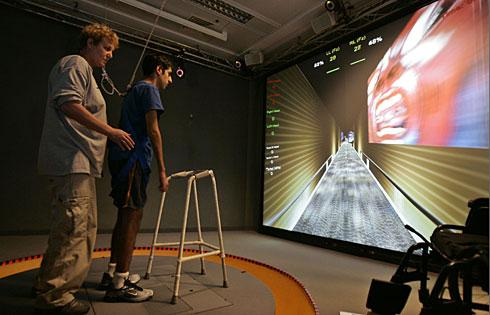
\includegraphics[scale=0.8]{../images/rehab_example.JPG} 
\label{img:example}
\caption{Shalev Malki - disabled patient in Israel, using a virtual reality system to control a video game, that forces him to use atrophied muscles. From Chaim Sheba Medical Center, Tel Hashomer, 2006}
\end{figure}

The treatment, depending on symptoms and severity of the CP may consist of classic physical therapy (most important), occupational therapy, recreational therapy (improves physical and cognitive skills), speech and language therapy and more, depending on child needs. It may be combined with oral medication, used to relax stiff, contracted, or overactive muscles. Surgeries may be performed in order to help with orthopedic problems or to cut nerves to reduce chronic pain and severe spasticity.

\subsection*{Motivation}

As it was previously mentioned, different types of physical therapy are important part of supporting treatments. For some time already \cite{rehabilitation}, modern healthcare started including \emph{serious games}. \emph{Serious game} is a name for a broad genre of video games that are designed for purpose other than pure entertainment, e.g. learning, rehabilitation, information spreading. In medicine, they are used as a part of educational process \cite{exercise}, mental therapies \cite{mental_game, mental}, or rehabilitation \cite{physical_rehab, stroke_rehab}. 

Results of such experiments are promising - subjects are more willing to participate in exercises and also learn faster when enjoying the game. Enjoyment is an important factor in children rehabilitation, who often lack motivation or perseverance to perform exercise every day. 

It seems like a natural consequence to build a serious game that can help with one of the typical children disorders - cerebral palsy. The part of rehabilitation especially important for this group is hand-eye coordination.

\subsection*{State of the art}
There are some existing solutions and they are mostly using custom controller\cite{game_custom}, that are expensive and/or not in serial production or XBox Kinect \cite{game_xbox_360} which is not a precise tool and works better for overall body rehabilitation. 

\subsection*{Project scope}
In last years, a lot of new commercially available controllers entered the market (e.g. \cite{Leap}, \cite{TheEyeTribe}), that may be better and cheaper  than existing solution, especially for aim of creating eye-hand coordination games. First, a CP study should be made, with focus on which age group and CP severity level can be the best recipient of the application. Then, using factors and parameters obtained from previous part, the detailed analysis of available hardware (controllers) and software (eye and hand movement detection from video stream) will be performed to find the optimal solution.
Later, one or more prototype will be prepared, using this solutions and tested on children. The results will be evaluated to check if the analysis assumptions were correct or not. 

\section*{Plan for the next weeks}

\begin{enumerate}
\item Detailed analysis of the topic: cerebral palsy, available controllers and software
\item Prototyping
\item Testing
\end{enumerate}


\bibliographystyle{plain} 
\bibliography{../references/references}

\end{document}
